%\documentclass[onecolumn,draftcls]{IEEEtran}
%\documentclass[journal,twocolumn,10pt,letter]{IEEEtran}
%\documentclass[conference,10pt,twocolumn,letter]{IEEEtran}
\documentclass[journal,onecolumn,11pt,draftcls,doublespace]{IEEEtran}
%\documentclass[journal,onecolumn,11pt,doublespace]{IEEEtran}
%\documentclass[journal,onecolumn,11pt,draftcls,doublespace]{IEEEtran}
%\documentclass[journal,onecolumn]{IEEEtran}
\IEEEoverridecommandlockouts
\ifCLASSINFOpdf
\else
\fi
\usepackage{algorithm}
\usepackage[noend]{algpseudocode}
\usepackage[cmex10]{amsmath}
\usepackage{amsthm}
\usepackage{amssymb}
\usepackage{mathrsfs}
\usepackage{amsbsy}
\usepackage{mathrsfs}
\usepackage{setspace}
\usepackage{graphicx}
\usepackage{caption}
\usepackage{subcaption}
\usepackage{psfrag}
\usepackage{newclude}
\usepackage[normalem]{ulem}
\usepackage{latexsym}
%\usepackage{tikz}
\usepackage[table]{xcolor}
\usepackage{multirow}
\usepackage{rotating}
\usepackage{booktabs}
\usepackage{amsmath}
\usepackage{mathrsfs}
\usepackage{bbm} % indicator function
\usepackage{filecontents}
\usepackage{amsmath,epsfig,cite,amsfonts,amssymb,psfrag,subfig}
\def\CE{\mathcal{E}}
\def\A{{A^n_\epsilon}}
\def\bS{{\boldsymbol{S}}}
\def\bs{{\boldsymbol{s}}}
\def\bz{{\boldsymbol{z}}}
\def\bu{{\boldsymbol{u}}}
\def\bv{{\boldsymbol{v}}}
\def\bU{{\boldsymbol{U}}}
\def\bx{{\boldsymbol{x}}}
\def\bX{{\boldsymbol{X}}}
\def\by{{\boldsymbol{y}}}
\def\bY{{\boldsymbol{Y}}}
\def\pr{{\text{P}}}
\def\c{{\mathcal{C}}}
%%%%%%%%%%%%%%%%% Define \doublehat
\usepackage{accents}
\usepackage[absolute]{textpos}
\newlength{\dhatheight}
\newcommand{\doublehat}[1]{%
    \settoheight{\dhatheight}{\ensuremath{\hat{#1}}}%
    \addtolength{\dhatheight}{-0.35ex}%
    \hat{\vphantom{\rule{1pt}{\dhatheight}}%
    \smash{\hat{#1}}}}
%%%%%%%%%%%%%%%%%%% Define Independent Symbol
\newcommand\independent{\protect\mathpalette{\protect\independenT}{\perp}}
\def\independenT#1#2{\mathrel{\rlap{$#1#2$}\mkern2mu{#1#2}}}
%%%%%%%%%%%%%%%%%%%%%%%%%%%
\allowdisplaybreaks
\newtheorem{remark}{Remark}
\newtheorem{theorem}{Theorem}
\newtheorem{lemma}{Lemma}
\newtheorem{proposition}{Proposition}
\newtheorem{corollary}{Corollary}
\graphicspath{{figures/}}
\allowdisplaybreaks
\newcommand{\eqdef}{\overset{\mathrm{def}}{=\joinrel=}}
\hyphenation{op-tical net-works semi-conduc-tor}
%%%%%%%%%%%%%%%%%%%%%%%%%%%%%%%%%%%%%%%%%%%%%%%%%%%%%%%%%%%%%%%%%%%%%%%%%%%%%%%%%%%%%%%%%%%%%%%%%%%%%%%%%%%%%%%%%%%%%%%%%%%%%%%%%%%%
\begin{document}

\title{"In the name of GOD" \\[2in] Power Allocation for Distributed MIMO C-RAN System } \author{\IEEEauthorblockN{\normalsize
     Mojdeh Karbalaee Motalleb}

    \vspace{2cm}
    }

\maketitle

\newpage
%%%%%%%%%%%%%%%%%%%%%%%%%%%%%%%%%%%%%%%%%%%%%%%%%%%%%%%%%%%%%%%%%%%%%%%%%%%%%%%%%%%%%%%%%%%%%%%%%%%%%%%%%%%%%%%%%%%%%%%%%%%%%%%%%%%%
\begin{abstract}
Cloud radio access networks generate a new architechture for 5G that is proposed to enhance both spectral efficiency and energy efficiency. 
This project investigates the optimal power allocation for the downlink of Multiple-Input Multiple-Output (MIMO) Cloud Radio Access Network (C-RAN) with limited fronthaul capacity in terms of maximizing Energy Efficiency (EE). 
In the considered system, the compressed and precoded message generated by Central Unit (CU) is transmitted to Remote Radio Heads (RRHs) via a fronthaul link with limited capacity, and the RRHs and Users Equipments (UEs) are assumed to be clustered into $S$ cluster sets.
Here, we use an iterative algorithm with Lagrangian function to optimize the EE.


 \emph{index Terms}- Cloud Radio Access Network, Multiple-Input Multiple-Output, Energy efficiency, Clusterization, Power allocation, Lagrangian function.
\end{abstract}
\IEEEpeerreviewmaketitle
%%%%%%%%%%%%%%%%%%%%%%%%%%%%%%%%%%%%%%%%%%%%%%%%%%%%%%%%%%%%%%%%%%%%%%%%%%%%%%%%%%%%%%%%%%%%%%%%%%%%%%%%%%%%%%%%%%%%%%%%%%%%%%%%%%%%
\newpage
\tableofcontents
\newpage
\listoffigures
\listoftables
\newpage
\section{Introduction}
The growing demand of higher data rates led vendors to think of the next generation of wireless networks which will essentially provide higher throughputs and more coverage than the state-of-art technologies. There are some new concepts introduced to enhance 5G networks such as; Het-Net systems, mmWave communications, Large-scale MIMO systems, and Cloud-Radio Access Networks. Each of the above mentioned concepts fulfills different requirements of 5G networks. As the main focus of this project is on the C-RAN technology, it is briefly introduced next. In C-RAN systems, in order to have a more efficient system in terms of computational resources, baseband processings, which may have high computational complexities, are transfered from base stations to control centers located in a cloud. In addition to manage computational resources, C-RAN technology can provide new concepts such as co-operation among RRHs, RRH clustering \cite{33,55}. To obtain both advantages of C-RAN and MIMO system, using MIMO C-RAN system simultaneously can enhance achievable rate and also EE \cite{33}. By using MIMO system, we can achieve higher data rates and even better EE compared to conventional systems by exploiting multiple number of antennas to transmit or receive data streams.


In order to consider feasible links between CU and RRHs, named as \emph{fronthaul}, the capacities of these links are assumed to be limited \cite{22,44,1111,66}. As a result of the limited fronthaul capacity the signals passed through these links need to be compressed \cite{22,44,1111,66} . One of the main problems that recently has attracted the attention of researches in MIMO C-RAN systems is how to efficiently perform detections, precodings and compressions of messages before transmitting them to CU or RRHs. Deploying efficient resource allocations causes prevention of wasting energy and as a result leads to higher EE \cite{33,55,77}. In\cite{22,44,1111,66}, the authors investigated optimizing achievable rate according to the precoding and power matrix and quantization noise with fronthaul capacity constraint. In \cite{66}, the approach of CFE (Compress-Forward Estimate) in uplink (UL) and improving data rates is investigated by using ECF (Estimate-Compress-Forward) instead can reach better performance in system, where RRH, estimates CSIT in UL, compress message and forward it to CUs studied.
\begin{figure}[t]
  \centering
    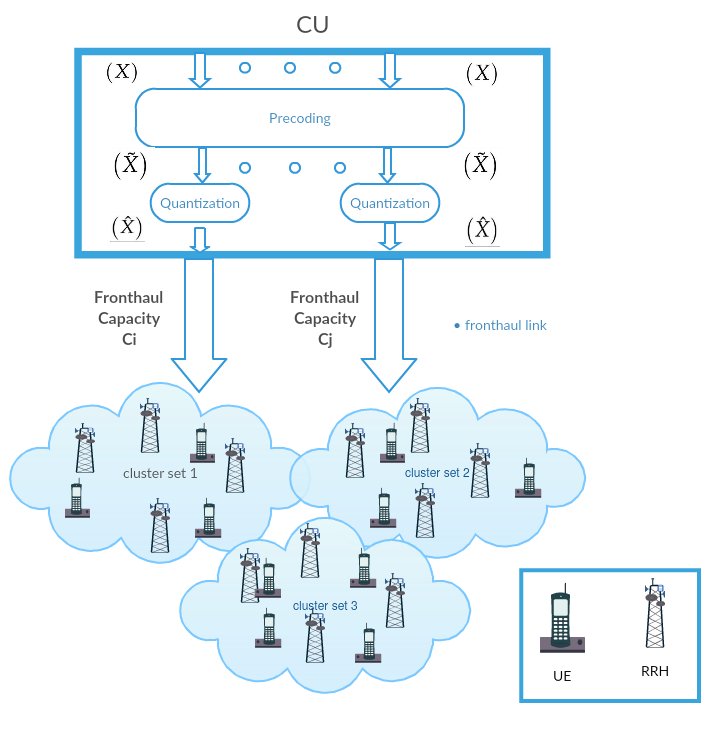
\includegraphics[width=8cm, height=8cm]{c1}
  \caption{Cooperative MIMO downlink C-RAN system.}
  \label{fig:c11}
\end{figure}

In this project, the downlink of a MIMO C-RAN system is considered where CU precodes the message, and then compresses the resulting signals. The compressed version of the signal is transmitted over the limited capacity fronthaul links to the RRHs. It is assumed that RRHs and UEs are clustered in a way that several clustered RRHs serve certain groups of UEs. In such a system the knowledge of Channel State Information at Transmitter (CSIT) is needed to compute the precoding matrices. Since CSIT is imperfectly obtained from the uplink pilot transmissions, we assume that the CSIT is obtained with a certain estimation error. At the CU, the well known Minimum Mean Square Error (MMSE) precoding MMSE is applied to reduce multi-user interference and enhance the performance of the system. For the proposed downlink system, we firstly derive the achievable rate subject to the fronthaul capacity constraint, then we optimize the power allocation to maximize the energy efficiency. The improvement over the equal power allocation is highlighted through numerical discussions. For the proposed down link system, we firstly derive the achievable rate subject to the fronthaul capacity constraint, then we optimize the power allocation to maximize the energy efficiency. The improvement over the equal power allocation is highlighted through numerical discussions.

The project is organized as follows.The C-RAN system is expressed in Section II. Section III, expressed  research exprerienced and classification. Criticizing and comparing the papers is presented in Section IV .System model, achievable rate analysis and problem formulations are presented in Section V. Optimization problems are considered in Section VI. Section VII presents numerical results and discussions, and finally the project is concluded in Section VII.
\section{C-RAN}
C-RAN architecture is a new architecture that may be used in next generation of mobile cellular network.
since now, there are two other mobile architecture that is expressed in below.
  \begin{figure}
  \centering
    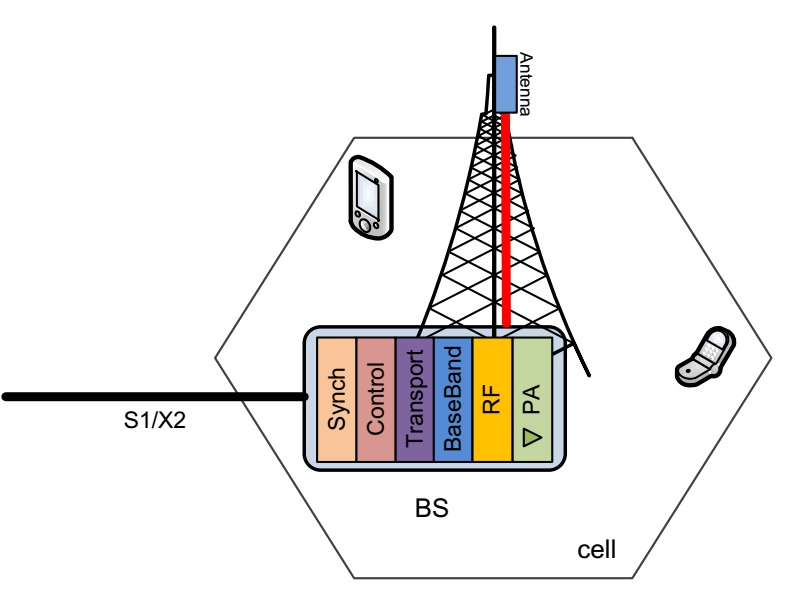
\includegraphics[width=0.5\linewidth, height=6cm]{trad}
  \caption{Traditional architecture \cite{369}}
  \label{fig:trad}
\end{figure}
\subsection{Traditional architecture}
In this architecture, radio processing and base band processing are merging together in a base station.
The module of antenna is generally located in the proximity (few meters) of
the radio module as shown in Figure \eqref{fig:trad} as coaxial cables
employed to connect them exhibit high losses.
This architecture was
used for 1G and 2G mobile networks \cite{369}.
%%


\subsection{Base station with RRH}
In this architecture, the base station is contained of a radio unit and a
signal processing unit, as shown in Figure \eqref{fig:rrh} . The radio unit
is called a RRH or Remote Radio Unit (RRU). RRH provides
the interface to the fiber and performs digital processing,
digital to analog conversion, analog to digital conversion,
power amplification and filtering. The baseband signal
processing part is called a BBU. This architecture is used for 3G  and 4G networks.
\begin{figure}
  \centering
    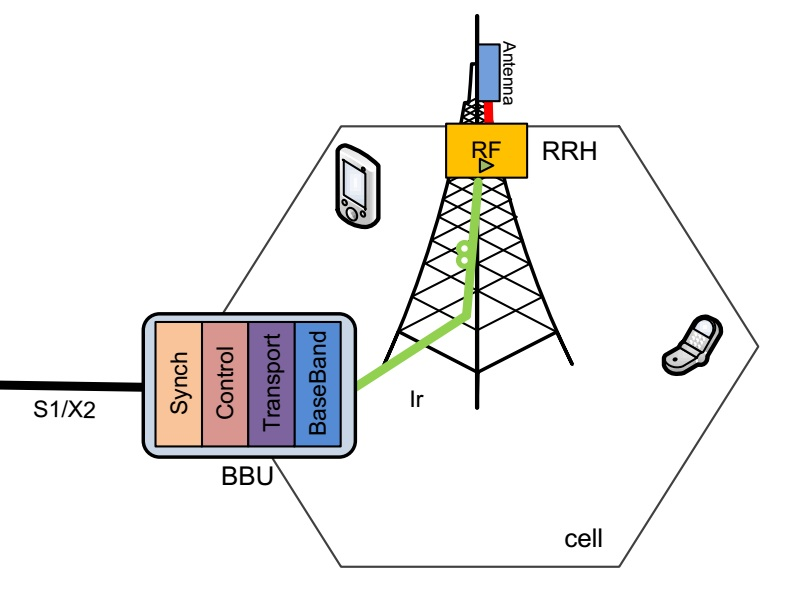
\includegraphics[width=0.5\linewidth, height=6cm]{rrh}
  \caption{Base station with RRH architecture \cite{369}}
  \label{fig:rrh}
\end{figure}
The distance between a RRH and a BBU  can be about 40 km since there is a limitation for delay and processing it can not be longer.
Optical fiber and microwave connections
can be used.
Also One BBU can servemany RRHs \cite{369}.
\subsection{C-RAN Architecture}
In this architecture, the BBUs are centralized into one entity that is called a BBU/DU Pool, for optimizing BBU utilization between
heavily and lightly loaded base stations.
A BBU Pool is shared between cell sites and virtualized as
shown in Figure \eqref{fig:cr}. A BBU Pool is a virtualized cluster which
can consist of general purpose processors to perform baseband
(PHY/MAC) processing. 
\begin{figure}[H]
  \centering
    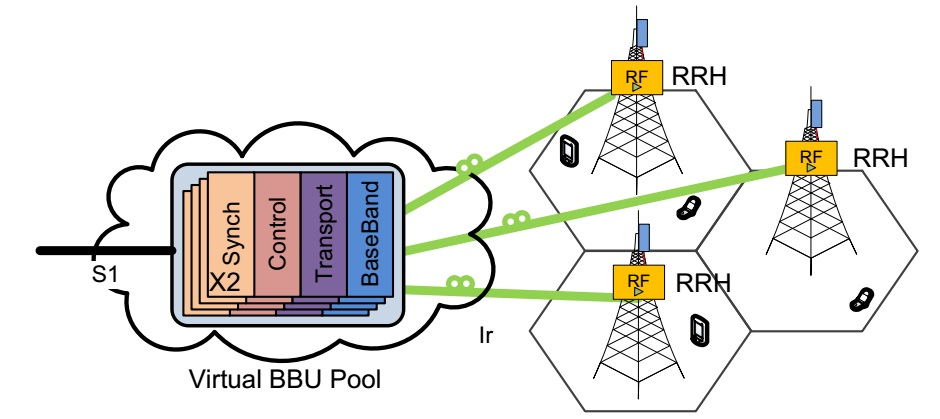
\includegraphics[width=0.5\linewidth, height=6cm]{cr}
  \caption{C-RAN architecture \cite{369}}
  \label{fig:cr}
\end{figure}
The concept of C-RAN was first introduced by IBM 
under the name Wireless Network Cloud (WNC) and builds
on the concept of Distributed Wireless Communication System.
Here, a user communicates with densely placed distributed
antennas and the signal is processed by Distributed Processing \cite{369}.
\section{Research Experience and Classification}
In this part we compare studied papers in downlink.
Nowadays many researches includes MIMO system in C-RAN architecture.
These papers which I have studied (which are expressed in downlink) separated in 3 groups.
\subsection{First group}
In uplink, we have 2 part that separate time in 2 section. First portion of time is for sending pilot and second portion is for sending message that we do not discuss it. 
In downlink they have used precoding and compression in transmitter \cite{22,1111,44,66}. 
The equations is represented as 
\begin{equation}
\label{eq_pow1}
 \hat{\boldsymbol{x}} = \tilde{\boldsymbol{x}} + \boldsymbol{Q},
\end{equation}
where, $\boldsymbol{Q} = \left[ q_,\ldots,q\right]^T$,  is the quantization noise vector originating from compression made after precoding in the CU with element distribution of
$q\backsim \mathcal{N}(0,\sigma_{q^2}) $. Moreover,
$$\tilde{\boldsymbol{x}} = \textbf{W}\textbf{P}^{\frac{1}{2}} \boldsymbol{x},$$
\begin{figure}[H]
  \centering
    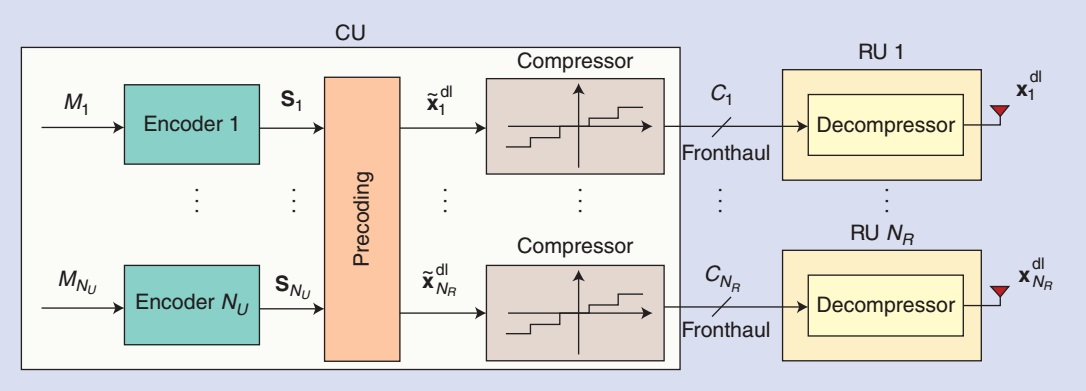
\includegraphics[width=\linewidth, height=6cm]{dl}
  \caption{First group of C-RAN architecture \cite{1111}}
  \label{fig:dl}
\end{figure}
denotes the precoded message before compression and $\boldsymbol{x}$ denotes the original message.
Fig \eqref{fig:dl} has shown this structure. In this group they have already maximized rate subject to a limitation on capacity of fronthaul link and power of transmitter.
The optimization formulation is denoted as 
\begin{equation}
\begin{aligned}
\max\limits_{\boldsymbol{W},\boldsymbol{\sigma}}   \quad &   \sum R(\boldsymbol{W},\boldsymbol{\sigma})\\
\text{subject to} \quad  & \bar{p}(\boldsymbol{W}, \boldsymbol{\sigma}) \leq P_{max}   \\
&C(\boldsymbol{W},\boldsymbol{\sigma})\leq C^{th}  \\
\end{aligned}
\end{equation}
where $\boldsymbol{\sigma}$ is variance of quantization noise and $\boldsymbol{W}$ is precoding matrix. In this problem, we want to maximize rate subject to limitation for capacity of fronthaul link and limitation in power transmitted by each RRH. In this case, we solve the problem by using iterative algorithm. The iterative algorithm utilize Largrangian method to solve the problem so
it may be a centralized algorithm not distributed method. In section V, we have used these kinds of algorithms. Also the complete solution and algorithm for this problem can be found in \cite{22}.
\subsection{Second group}
In this group, the downlink MIMO systems with a C-RAN architecture is expressed \cite{33,55}. The problem is approxiomateley similar to system model introduced in section IV.
Here, RRHs and users are clustered to $S$ cluster. 
In this group, the recieved signal vector for each user in $s^{th}$ cluster can be demonstrate as 
\begin{equation} \label{sg}
\textbf{y}_{u_s} = \sum_{t=1}^S \textbf{G}_{M_t,u_s}^H \textbf{W}_{M_t,u_t} \textbf{P}_{u_t}^{\frac{1}{2}} \textbf{x}_{ u_t} + \textbf{z}_{U_S}
\end{equation}
where $\textbf{x}_{ u_t} = [x_{ u_{(t,1)}},..., x_{ u_{(t,U_t)}}]^T \in C^{ U_t \times T} $ is the transmit symbol vector of RRH cluster $t$ that $T$ is symbol duration. 
 $\textbf{W}_{M_t, u_t} = [w_{ M_t,u_{(t,1)}},..., w_{M_t, u_{(t,U_t)}}]^T \in C^{ M_t \times U_t} $ is the precoding matrix exerted to RRHs  and users in $t^th$ cluster.
 Moreover, $\textbf{G}_{M_t,u_s}$ is the channel gain from RRH set $M_t$ to user set $U_s$. In addition, $z_{U_s}$ is the additive guassian noise.This problem is identical to our problem statement in section IV. The difference is that we do not use compression here. System model is also same as system model in section IV with constraint of
   $\boldsymbol{Q}_{\mathcal{R}_v} = \boldsymbol{0}$. The problem statement is a bit different from section V. The problem formulation is shown as below \cite{33}
   \begin{equation}\label{p12}
\begin{aligned}
\max\limits_{\boldsymbol{P}}   \quad &   \eta(\boldsymbol{P})\\
\text{subject to} \quad  & \bar{p}_{u_{(s,k)}} \leq P_{max} && \qquad \forall s, \forall i,   \\
&\mathfrak{R}_{u_{(s,k)}} \geq  \mathfrak{R}_{u_{(s,k)}}^{th} && \qquad \forall s, \forall k, \\
&p_{u_{(s,k)}}  \geq 0                                  &&\qquad \forall s, \forall k, \\
\end{aligned}			
\end{equation}  
Where $\eta$ is the energy efficiency that is explained in later sections in equation \eqref{eta}. \\
In this problem, by using Lagrangian method and also iterative algorithm the problem is solved. Also some simplified method will be used here that is denoted in later sections.


For extending this problem statements, joint clusterization and power allocation is considered \cite{55}. This problem used the system model as shown below but there is a slight difference between it and equation \eqref{sg}.
The recieved signal for $k^{th}$ user can be formulated as 
\begin{equation} \label{sg1}
\begin{aligned}
\textbf{y}_{k} =& \sum_{c=1}^C \sum_{m=1}^M  \phi_{c,m,k}h_{m,k}w_{m,k} \sqrt{p_k x_k} \\
&+ \sum_{c=1}^C \sum_{m=1}^M \sum_{r=1 ,r \neq k}^K  \phi_{c,m,r}h_{m,k}w_{m,r} \sqrt{p_r x_r} + n_k,
\end{aligned}	
\end{equation}
where,  $h_{m,k}$ is the channel gain between $k^{th}$ user and $m^{th}$ RRH. What's more, $w_{m,k}$ is the precoding between $k^{th}$ user and $m^{th}$ RRH. Additionally, $p_k$ is the 
transmit symbol power and $x_k$ is the transmit symbol of $k^{th}$ user. On top of them, $ \phi_{c,m,k} \in {0,1}$ and it is 1 if $k^{th}$ user and $m^{th}$ RRH are in the $c^{th}$ cluster, otherwise it is 0.  The problem statement  is maximizing energy efficiency with some constraints as below.
\begin{equation}
\begin{aligned}
\max\limits_{\boldsymbol{P},\boldsymbol{\phi}}   \quad &   \eta\\
\text{subject to} \quad  & \sum_{c=1}^C \sum_{k=1}^K  \phi_{c,m,k}|w_{m,k}|^2 p_k , \forall m,   \\
&\mathfrak{R}_{k} \geq  \mathfrak{R}_{k}^{th} && \qquad  \forall k, \\
&p_{k}  \geq 0                                  &&\qquad  \forall k, \\
& \phi_{c,m,k} \in \{0,1\} \\
 &\sum_{t=1, t \neq c}^C \sum_{m=1}^M  \phi_{c,m,k}\sum_{m=1}^M \phi_{t,m,k} \leq 0    &&\qquad    \forall m  , \forall c, \\
  &\sum_{t=1, t \neq c}^C \sum_{k=1}^K  \phi_{c,m,k}\sum_{k=1}^K \phi_{t,m,k} \leq 0      &&\qquad      \forall m  , \forall c,\\
  &\sum_{k=1}^K \sum_{m=1}^M  \phi_{c,m,k} \geq 1\\
\end{aligned}	
\end{equation}
Here, by exerting Lagrangian function or method and deriving, the problem will be solved. To maximize energy efficiency, we use Theorem \ref{t2} for simplicity. 
\subsection{Third group}
In this group, we have studied papers such as \cite{cell, 88}. In these papers, C-RAN architecture is not deployed. They are about MIMO systems. In this case, cell free system is employed. 
That large number of access point are serving small number of users. In uplink, the channel is separeted into 2 section. First for sending pilot and then for sending message. Here, the system model is completely distinct from the other system models. It is shown in below
\begin{equation}
y_k = \sqrt{\rho}\sum_{k'=1}^K g_{m_{k'} k} \sqrt{\alpha_{k'} q_{k'}} + n_k
\end{equation}   
where, $\sqrt{\alpha_{k'} q_{k'}}$ is the message signal. Additionally, $\sqrt{\rho}$ is the normalized SNR and $n_k$ is additive noise. Also $ g_{m_{k'} k}$ is channel gain from $m_{k'}$ access point to $k$ user. In this case, maximizing the minimum rate is considered. 
   \begin{equation}
\begin{aligned}
\max\limits_{\alpha_k}   \quad & min \quad  R_k\\
\text{subject to} \quad  & 0\leq \alpha_k \leq 1, && \qquad \forall k \in \{1,...,K\}  \\
\end{aligned}			
\end{equation}
 \section{Criticizing and Comparing Existing Papers}
 \subsection{Difference in System models}
 In this section we want to summerize the system models and methods in downlink and compare them. In the first group, compression and precoding is deployed in downlink. Firstly, message is encoded. after that it is precoded by CU (BBU Pool), then the precoded message is quantized and after that it is transmitted through fronthaul link with constrained capacity which is 
 depended on precoding and quantization noise
 to RRHs by fiber link. Finally it will be transmitted by RRHs through wireless link to users. Here, RRHs and users are not clustered.
  In second group the message is just encoded and precoded and then transmit through fronthaul link which has unconstrained capacity to RRHs which are clustered and finally it is transmitted  by RRHs through wireless link to users. Here quantization noise is not considered but RRHs and users are clustered.
  In the third group, we have expressed cell free massive MIMO. It is just new idea and we do not use it here a lot. 
  In the first group, RRHs and users are not clustered and in the second group, quantization noise is not exerted. In next section, we present new system model that has both quantization noise and clustering. 
  \subsection{Similarity and difference in problem statements}
  In all 3 groups, they have defined optimization problem which is about power allocation. In first group, maximizing sum rate is discussed. In second group maximizing energy efficiency  assumed also contains
   maximizing rate. In third group, maximizing the minimum rate is investigated. By maximizing minimum rate, all other rates are also enhanced. 
   All 3, try to maximize wireless channel rate in some ways subject to power contraints. In the first group we have also limitation on capacity. In the second group we have discussed about joint clustering and power allocation too. In first and second group, the problem is solved by both iteration algorithm and Lagrangian function together. Since it is discussed in downlink. the methods are approximately centralized.
 
   
   In next section, we have tried to merge all three groups together.
\section{System Model and Problem Formulation}

In this section, the system model, achievable rate and the main problem which is optimizing power allocation is expressed.

\subsection{System Model}

Downlink of a MIMO C-RAN system consists of $R$ RRHs serving $D$ single antenna user equipments (UE) is considered. It is assumed that RRHs and UEs are clustered in to $S$ cluster sets such that the $v$-th cluster set, has $R_v$ RRHs serving ${D}_v$ UEs. Furhtermore, it is assumed that the $j$-th RRH in the $v$-th cluster is connected to the CU via an optical fiber link with a limited capacity of $c_{r_{(v,j)}}$. So, we have
\begin{equation}
\begin{split}
\mathcal{R}_v= \{  r_{(v,i)} | 1 \leq i \leq {R}_v , i\in Z^+\}, \\
\mathcal{C}_{\mathcal{R}_v}= \{c_{r_{(v,j)}}| 1 \leq j \leq {R}_v , j\in Z^+\}, \\
\mathcal{D}_v= \{  d_{(v,k)} | 1 \leq k \leq {D}_v , k\in Z^+\},  \\
\end{split}
\end{equation}
where $\mathcal{R}_v$, $\mathcal{C}_{\mathcal{R}_v}$, and $\mathcal{D}_v$ respectively represent the RRH set, the capacity set and the UE set  for the $v$-th cluster set.
In CU we apply the approach of compressing after precoding and then forwarding. Each user receives both intra-cluster and inter-cluster interferences.
\subsection{Achievable Rate Analysis}
In this subsection, the achievable data rate of the considered system is investigated. 
\begin{theorem}\label{t1}
The achievable data rate for UE $d_{(s,k)}$ is
\begin{equation}\label{e1}
\mathfrak{R}_{d_{(s,k)}} = B \log_2(1+\gamma_{d_{(s,k)}}),
\end{equation}
where, $B$ is the channel bandwidth and $\gamma_{d_{(s,k)}}$ is the received SINR for the $k$-th UE in the $s$-th cluster set which is formulated as
\begin{equation}\label{5}
\gamma_{d_{(s,k)}}= \frac{p_{d_{(s,k)}}|\boldsymbol{h}_{\mathcal{R}_s, d_{(s,k)}}^H \boldsymbol{w}_{\mathcal{R}_{s},d_{(s,k)}}|^2}{I_{d_{(s,k)}}+BN_0}.
\end{equation}
In \eqref{5}, $I_{d_{(s,k)}}$, denotes the power of interfering signals, $BN_0$ represents the noise power, $\boldsymbol{h}_{\mathcal{R}_s, d_{(s,k)}}$ shows the channel gain vector between the $k$-th UE and the RRHs in the $s$-th cluster set, and $\boldsymbol{w}_{\mathcal{R}_{s},d_{(s,k)}}$ indicates the precoding vector used in $s$-th cluster set for the $k$-th UE.
$p_{d_{(s,k)}}$ is the transmit power of RRHs that transmit to the $k$-th UE in the $s$-th cluster set.
\end{theorem}

\begin{proof}
%%%%%%%%%%%%%
Let $\boldsymbol{y}_{\mathcal{D}_s}$ be a $D_s \times 1$ vector denoting the received signals by the set of UEs in the $s$-th cluster which is given by
\begin{equation} \label{1}
\boldsymbol{y}_{\mathcal{D}_s} = \sum_{v=1}^S \boldsymbol{H}^H_{\mathcal{R}_v,\mathcal{D}_s}\hat{\boldsymbol{x}}_{\mathcal{R}_v}+ \boldsymbol{z}_{\mathcal{D}_s},
\end{equation}
where $\hat{\boldsymbol{x}}_{ \mathcal{R}_v} = [\hat{x}_{ r_{(v,1)}},...,\hat{ x}_{ r_{(v,\mathcal{R}_v)}}]^T \in \mathbb{C}^{{R}_v } $ is the transmitted symbol vector for the $v$-th cluster set, $\boldsymbol{z_{\mathcal{D}_s}} \backsim \mathcal{N}(0,N_0\boldsymbol{I}_{{D}_s})$ shows the additive White Guassian noise with the power of $N_0$, and $\boldsymbol{H}_{\mathcal{R}_v,\mathcal{D}_s}=\left[\boldsymbol{h}_{\mathcal{R}_v,d_{(s,1)}},\ldots,\boldsymbol{h}_{\mathcal{R}_v,d_{(s,\mathcal{D}_s)}}\right]^T  \in \mathbb{C}^{{R}_v\times {D}_s}$ 
represents the channel matrix between RRH set $\mathcal{R}_v$ to UE set
$\mathcal{D}_s$. The channel vector from the RRH cluster $v$ to the $k$-th UE in the $s$-th cluster set $\boldsymbol{h}_{\mathcal{R}_v,d_{(s,k)}}\in \mathbb{C}^{{R}_v}$ is modeled as follows
\begin{equation}
\boldsymbol{h}_{\mathcal{R}_v,d_{(s,k)}} = \boldsymbol{\beta}^\frac{1}{2}_{\mathcal{R}_v,d_{(s,k)}} \boldsymbol{g}_{\mathcal{R}_v,d_{(s,k)}},
\end{equation}
% resizebox{0.3\hsize}{!}{$
where $\boldsymbol{g}_{\mathcal{R}_v,d_{(s,k)}} \backsim \mathcal{N}(0,N_0\boldsymbol{I}_{\mathcal{D}_s})$ represents the fast and flat fading channel vector and $\boldsymbol{\beta}_{\mathcal{R}_v,d_{(s,k)}}=\text{diag}(a_{r_{(v,1),d_{(s,k)}}},\ldots,a_{r_{(v,\mathcal{R}_v),d_{(s,k)}}})$
indicates the large scale fading matrix \cite{88}. In addition, the transmitted signal has the following form
\begin{equation}
\label{eq_pow1}
 \hat{\boldsymbol{x}}_{\mathcal{R}_v} = \tilde{\boldsymbol{x}}_{\mathcal{R}_v} + \boldsymbol{Q}_{\mathcal{R}_v},
\end{equation}
where, $\boldsymbol{Q}_{\mathcal{R}_v} = \left[ q_{r_{(v,1)}},\ldots,q_{r_{(v,R_v)}}\right]^T$,  is the quantization noise vector originating from compression made after precoding in the CU with element distribution of
$q_{M_{(t,i)}}\backsim \mathcal{N}(0,\sigma_{q_{(t,i)}}^2) $. Moreover,
$$\tilde{\boldsymbol{x}}_{\mathcal{R}_v} = \textbf{W}_{\mathcal{R}_v,\mathcal{D}_v} \textbf{P}_{\mathcal{D}_v}^{\frac{1}{2}} \boldsymbol{x}_{ \mathcal{D}_v},$$
denotes the precoded message before compression.


As mentioned before, channel vector is assumed to be known with errors, the imperfection of channel estimation is modeled as follows
\begin{equation*}
\hat{\boldsymbol{h}}_{\mathcal{R}_v,d_{(s,k)}} = \boldsymbol{h}_{\mathcal{R}_v,d_{(s,k)}} + \Delta \boldsymbol{h}_{\mathcal{R}_v,d_{(s,k)}},
\end{equation*}
$\Delta \boldsymbol{h}_{\mathcal{R}_v,d_{(s,k)}}$ denotes the estimation error vector with a Guassian distribution of
$$\Delta \boldsymbol{h}_{\mathcal{R}_v,d_{(s,k)}}\backsim \mathcal{N}(0,\boldsymbol{\phi}_{\mathcal{R}_v,d_{(s,k)}}^2),$$
where 
$$\boldsymbol{\phi}_{\mathcal{R}_v,d_{(s,k)}} = \text{diag}(\phi_{r_{(v,1)},d_{(s,k)}},\ldots,\phi_{r_{(v,\mathcal{R}_v)},d_{(s,k)}}).$$


By using MMSE precoding, the precoding matrix is expressed as follows
\begin{equation}
\boldsymbol{W}_{\mathcal{R}_s,\mathcal{D}_s} = \hat{\boldsymbol{H}}_{\mathcal{R}_s,\mathcal{D}_s}(\hat{\boldsymbol{H}}_{\mathcal{R}_s,\mathcal{D}_s}^H \hat{\boldsymbol{H}}_{\mathcal{R}_s,\mathcal{D}_s}+ \alpha \boldsymbol{I}_{{D}_s})^{-1},
\end{equation} 
where, $\alpha$ is the regularization factor.


Therefore, the previously mentioned $I_{d_{(s,k)}}$, denoting the interference power at the desired UE in (3), can be written as follows
\begin{equation}\label{6}
\begin{split}
I_{d_{(s,k)}} &=  \underbrace{\sum_{\substack{l=1 \\ l\neq k}}^{{D}_s} |\boldsymbol{h}_{\mathcal{R}_s, d_{(s,k)}}^H \boldsymbol{w}_{\mathcal{R}_{s},d_{(s,l)}}|^2  p_{d_{(s,l)}}}_{\text{(intra-cluster interference)}}\\
&+\underbrace{\sum_{\substack{v=1 \\ v\neq s}}^{S} \sum_{l=1}^{{D}_s} |\boldsymbol{h}_{\mathcal{R}_v, d_{(s,k)}}^H \boldsymbol{w}_{\mathcal{R}_{v},d_{(v,l)}}|^2 p_{d_{(v,l)}}}_{\text{(inter-cluster interference)}}\\
& +\underbrace{ \sum_{v=1}^{S} \sum_{i=1}^{{R}_v} {\sigma_q}_{r_{(v,i)}}^2 \sum_{l=1}^{{D}_s} |\boldsymbol{h}_{r_{(v,i)}, d_{(v,l)}}^H|^2 }_{\text{(quantization noise interference)}}.
\end{split}
\end{equation}

 \end{proof}
\section{Optimizing Power Allocation}
Let the power of transmitted signal by the $i$-th RRH in the $s$-th cluster set by
\begin{equation} \label{eq_pow2}
\bar{p}_{r_{(s,i)}} = \mathit{E}[|| \hat{x}_{\mathcal{D}_v} ||^2],
\end{equation}
By plugging (\ref{eq_pow1}) into (\ref{eq_pow2}), the power of transmitted signal is rewritten as
\begin{equation}
\bar{p}_{r_{(s,i)}} = \boldsymbol{w}_{r_{(s,i)},\mathcal{D}_{s}} \boldsymbol{P}_{\mathcal{D}_v}^{\frac{1}{2}} \boldsymbol{P}_{\mathcal{D}_v}^{H \frac{1}{2}}   \boldsymbol{w}_{r_{(s,i)},\mathcal{D}_{s}}^H + \sigma_{q_{(s,i)}}^2.
\end{equation}
As a result the achievable rate on the fronthual link between the CU and the $i$-th RRH in $t$-th cluster must be larger than
\begin{equation}
C_{R_{(t,i)}} = \log{(1+\frac{w_{r_{(s,i)},\mathcal{D}_{s}} \boldsymbol{P}_{\mathcal{D}_v}^{\frac{1}{2}} \boldsymbol{P}_{\mathcal{D}_v}^{H \frac{1}{2}}   w_{r_{(s,i)},\mathcal{D}_{s}}^H }{ \sigma_{q_{(s,i)}}^2})},
\end{equation}
in order to be able to transmit the aforementioned signals via fronthual links.
\subsection{Problem Statement}
The ratio of the sum-rate of system to the total power transmitted by RRHs indicates one of the most pormising indicators for selecting new technologies, named as the energy efficiency of system and denoted by $\eta$, which can be formulated as
\begin{equation}\label{eta}
\eta(\boldsymbol{P}) := \frac{\sum\limits_{s=1}^{S} \sum\limits_{k=1}^{{D}_s}\mathfrak{R}_{d_{(s,k)}} }{\sum\limits_{s=1}^{S} \sum\limits_{i=1}^{{R}_s}\bar{p}_{r_{(s,i)}}} = \frac{R_{total}(\boldsymbol{P})}{P_{RRH}(\boldsymbol{P})},
\end{equation}
in which $ \boldsymbol{P} = \{ \boldsymbol{P}_{\mathcal{D}_s}|  1 \leq s \leq S, s \in \mathbb{Z}^{+} \}$ is a power allocation matrix.
In this project, maximization of energy efficiency is investigated with the presence of following constraints, 
\begin{equation}\label{p1}
\begin{aligned}
\max\limits_{\boldsymbol{P}}   \quad &   \eta(\boldsymbol{P})\\
\text{subject to} \quad  & \bar{p}_{r_{(s,i)}} \leq P_{max} && \qquad \forall s, \forall i,   \\
&\mathfrak{R}_{d_{(s,k)}} \geq  \mathfrak{R}_{d_{(s,k)}}^{th} && \qquad \forall s, \forall k, \\
&C_{r_{(s,i)}} \leq C_{r_{(s,i)}}^{th}  &&\qquad \forall s, \forall i, \\
&p_{d_{(s,k)}}  \geq 0                                  &&\qquad \forall s, \forall k, \\
\end{aligned}			
\end{equation}
Since the problem is not a convex problem, an iterative algorithm is used to derive the optimal values for the maximization problem. 
\subsection{Proposed Method}
In this subsection, instead of maximizing \eqref{eta}, we solve an equivalent problem by using an iterative algorithm. 
\begin{theorem}\label{t2}
Maximum value of $\eta^*$ is obtained if and only if 
\begin{equation}\label{q2}
\begin{split}
&\max \limits_{\boldsymbol{P}} (R_{total}(\boldsymbol{P}) - \eta^* P_{RRH}(\boldsymbol{P}))=\\
& R_{total}(\boldsymbol{P}^*) - \eta^* P_{RRH}(\boldsymbol{P}^*) =0,
\end{split}
\end{equation}
where $\{\boldsymbol{P}\}$ is a feasible solution of problem \eqref{p1}.
\end{theorem}
\begin{proof}
The Theorem is proved using the similar steps as [9, Theorem 1].
\end{proof}

To solve the optimization problem (14),, we use Lagrangian function  by an iterative algorithm proposed in \cite{11}.
For simplicity, the upper bound for the interference given in (9), is given by
\begin{equation}
\begin{split}
\tilde{I}_{d_{(s,k)}} &= \sum_{v=1}^{S} P_{max}|| \boldsymbol{h}_{\mathcal{R}_v,d_{(s,k)}} \boldsymbol{w}_{\mathcal{R}_v,d_{(s,k)}}||^2 ,\\
& +  \sum_{v=1}^{S} \sum_{i=1}^{{R}_v} {\sigma_q}_{r_{(v,i)}}^2 \sum_{l=1}^{{D}_s} |\boldsymbol{h}_{r_{(v,i)}, d_{(v,l)}}^H|^2.
\end{split}
\end{equation}
Therefore, to find the optimal power allocation, the following lower bound is used instead of (2), as
\begin{equation}\label{e11}
\mathfrak{\tilde{R}}_{d_{(s,k)}} = B \log_2(1+\tilde{\gamma}_{d_{(s,k)}}),
\end{equation}
where $\tilde{\gamma}_{d_{(s,k)}}$ is
\begin{equation}\label{15}
\tilde{\gamma}_{d_{(s,k)}} =  \frac{p_{d_{(s,k)}}|\boldsymbol{h}_{\mathcal{R}_s, d_{(s,k)}}^H \boldsymbol{w}_{R_{s},d_{(s,k)}}|^2}{\tilde{I}_{d_{(s,k)}}+BN_0};
\end{equation}

As mentioned before an iterative algorithm is used for optimization which is based on the following Lagrangian multiplier function
\begin{equation}
\begin{split}
\mathcal{L}(\boldsymbol{P}; \boldsymbol{\lambda}, \boldsymbol{\mu}, \boldsymbol{ \kappa}) & = \sum\limits_{s=1}^{S} \sum\limits_{k=1}^{\mathcal{D}_s}\mathfrak{\tilde{R}}_{d_{(s,k)}} 
- \eta \sum\limits_{s=1}^{S} \sum\limits_{i=1}^{\mathcal{R}_s}\bar{p}_{r_{(s,i)}}\\
&+\sum\limits_{s=1}^{S} \sum\limits_{k=1}^{\mathcal{D}_s} \lambda_{d_{(s,k)}} (\mathfrak{\tilde{R}}_{d_{(s,k)}}-\mathfrak{R}_{d_{(s,k)}}^{th})\\
&- \sum\limits_{s=1}^{S} \sum\limits_{i=1}^{\mathcal{R}_s} \mu_{r_{(s,i)}} (\bar{p}_{r_{(s,i)}}-P_{max})\\
&- \sum\limits_{s=1}^{S} \sum\limits_{i=1}^{\mathcal{R}_s} \kappa_{r_{(s,i)}} (C_{r_{(s,i)}}-C_{r_{(s,i)}}^{th}).\\
\end{split}
\end{equation}
where $\boldsymbol{\lambda}, \boldsymbol{\mu}, \boldsymbol{\kappa} \geq 0$ are Lagrangian multipliers vector.\\
By using this equation, the optimal power allocation is derived as below,
\begin{equation}
p_{r_{(s,i)}}^* =[\frac{ B(1+\gamma_{d_{(s,k)}} )}{\ln2 \times (\iota_{r_{(s,i)}}+ \chi_{r_{(s,i)}})} -\frac{\tilde{I}_{d_{(s,k)}} + BN_0}{\nu_{d_{(s,k)}} }]^+;
\end{equation} 
where $$\nu_{d_{(s,k)}} =|h_{\mathcal{R}_s, d_{(s,k)}}^H w_{R_{s},d_{(s,k)}}|^2,$$
 $$\iota_{r_{(s,i)}}=\sum\limits_{s=1}^{S} \sum\limits_{i=1}^{\mathcal{R}_s} (\mu_{r_{(s,i)}}+1)(w_{r_{(s,i)},d_{(v,l)}} w_{r_{(s,i)},d_{(v,l)}}^*),$$
 $$\chi_{r_{(s,i)}} \approx  \sum\limits_{s=1}^{S} \sum\limits_{i=1}^{\mathcal{R}_s} \frac{\kappa_{r_{(s,i)}}}{\ln 2}\frac{(w_{r_{(s,i)},d_{(v,l)}} w_{r_{(s,i)},d_{(v,l)}}^*)}{ \sum\limits_{k=1}^{\mathcal{D}_s}P_{max}+\sigma_{q_{r_{(s,i)}}}^2}.$$
  Finally, to find the optimal power allocation, the Algorithm I is applied. 
\begin{algorithm}
\caption{Energy-Efficient Power Allocation}\label{alg}
\begin{algorithmic}[1]
\State Set the maximum number of iterations $I_{max}$, convergence condition $\epsilon_{\eta}$  and the initial value $\eta^{(1)} = 0$
\State Set the iteration index $i = 1$ and begin the iteration (Outer
Loop).
\For {$ 1\leq i \leq  Imax$}
\State Solve the resource allocation problem with $\eta^{(i)}$ (Inner Loop);
\State Obtain $P^{(i)}, R_{total}^{(i)}, P_{RRH}^{(i)}$
\If {$ R_{total}(\boldsymbol{P}^{(i)}) - \eta^{(i)} P_{RRH}(\boldsymbol{P}^{(i)}) < \epsilon_{\eta} $} 
\State Set $\boldsymbol{P}^*= \boldsymbol{P}^{(i)} $   and  $ \eta^{*} =\eta^{(i)} $;
\State break;
\Else
\State Set $\eta^{(i)}= \frac{R_{total}(\boldsymbol{P}^{(i))}}{P_{RRH}(\boldsymbol{P}^{(i))}}$ and $i= i+1$;
\EndIf 
\State \textbf{end if}
\EndFor 
\State \textbf{end for}
\end{algorithmic}
\end{algorithm}
\section{Numerical Results and Discussions}
In this section, numerical results of the proposed algorithm are discussed for the MIMO C-RAN system whose parameters are described in Table \ref{tab:title}.

 \begin{table}[H]
 \caption {Simulation Parameter} \label{tab:title} 
 \begin{center}
  \begin{tabular}{||c c ||} 
  \hline
  Parameter & Value \\ [0.5ex] 
  \hline\hline
  Number of cluster S & 4 \\ 
  \hline
  Noise power & -174dBm/Hz\\
  \hline
  Bandwidth & 10MHz \\
  \hline
 Maxmimun transmit Power & 23dBm \\
  \hline
  Minimum data rate &  1Mbits/sec \\ [1ex] 
  \hline
 \end{tabular}
 \end{center}
 \end{table}
 
 
In Fig. \ref{fig:nem1},
energy efficiency of MIMO C-RAN system with the proposed iterative algorithm and equal power allocations are shown as a function of numbers of RRHs in each cluster.
As illustrated, optimal power allocation policy outperforms equal power allocation. In addition, it is shown that the increase in the number of RRHs enhances the performance of system.
 
  \begin{figure}
  \centering
    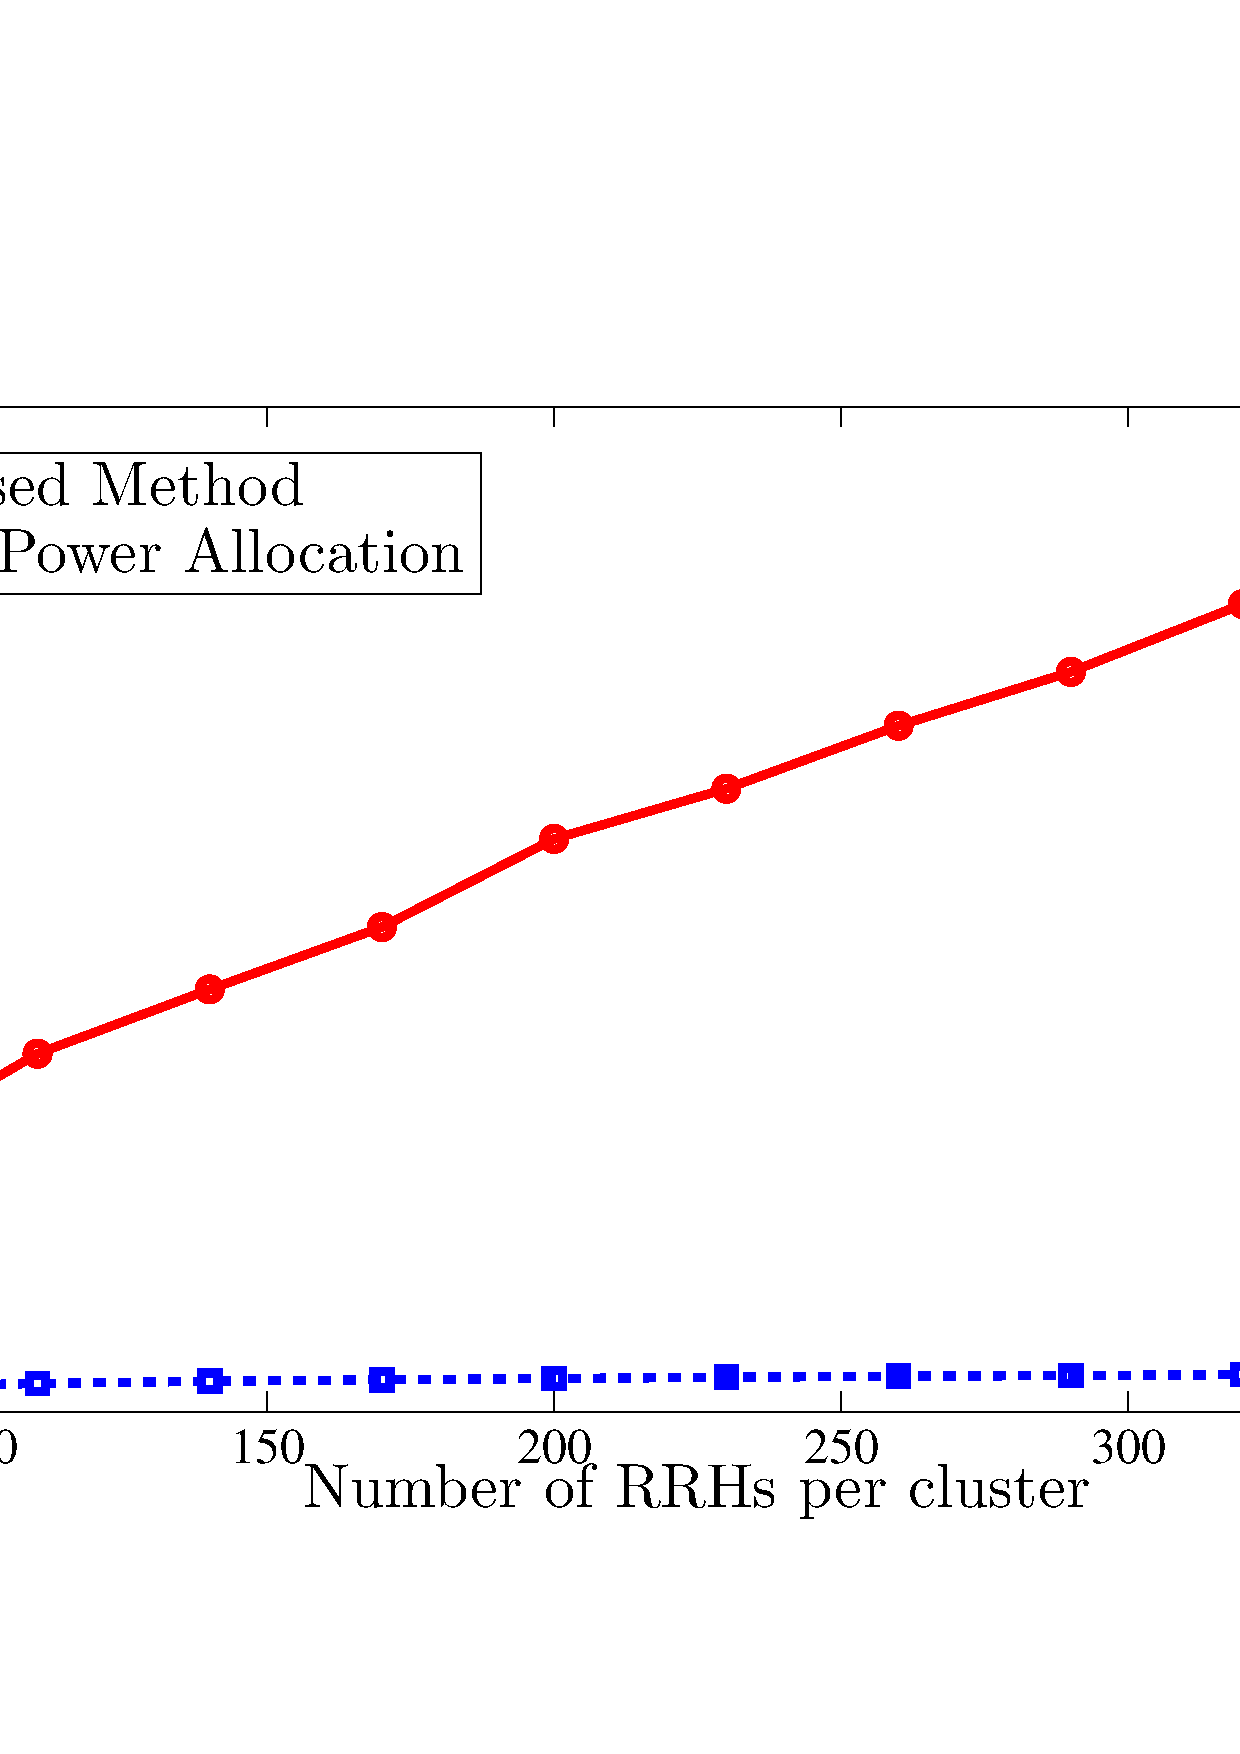
\includegraphics[width=0.5\linewidth, height=6cm]{n1232}
  \caption{Energy efficiency vs. number of RRH for optimal and equal power allocation. $U_s=8$, and the other parameters are given in Table I.}
  \label{fig:nem1}
\end{figure}


In Fig. \ref{fig:nem2}, EE of the proposed iterative algorithm and equal power allocation are depicted for different number of UEs in each cluster. Since by increasing the number of UEs in each cluster, interference is also increased, the system performance is decreased according to the increase in number of UE. It is shown that although the energy efficiency of the considered MIMO C-RAN systems degrades as the number of UEs increases, but still EE of the system using the proposed algorithm surpasses the equal power allocation.
  
  \begin{figure}
  \centering
    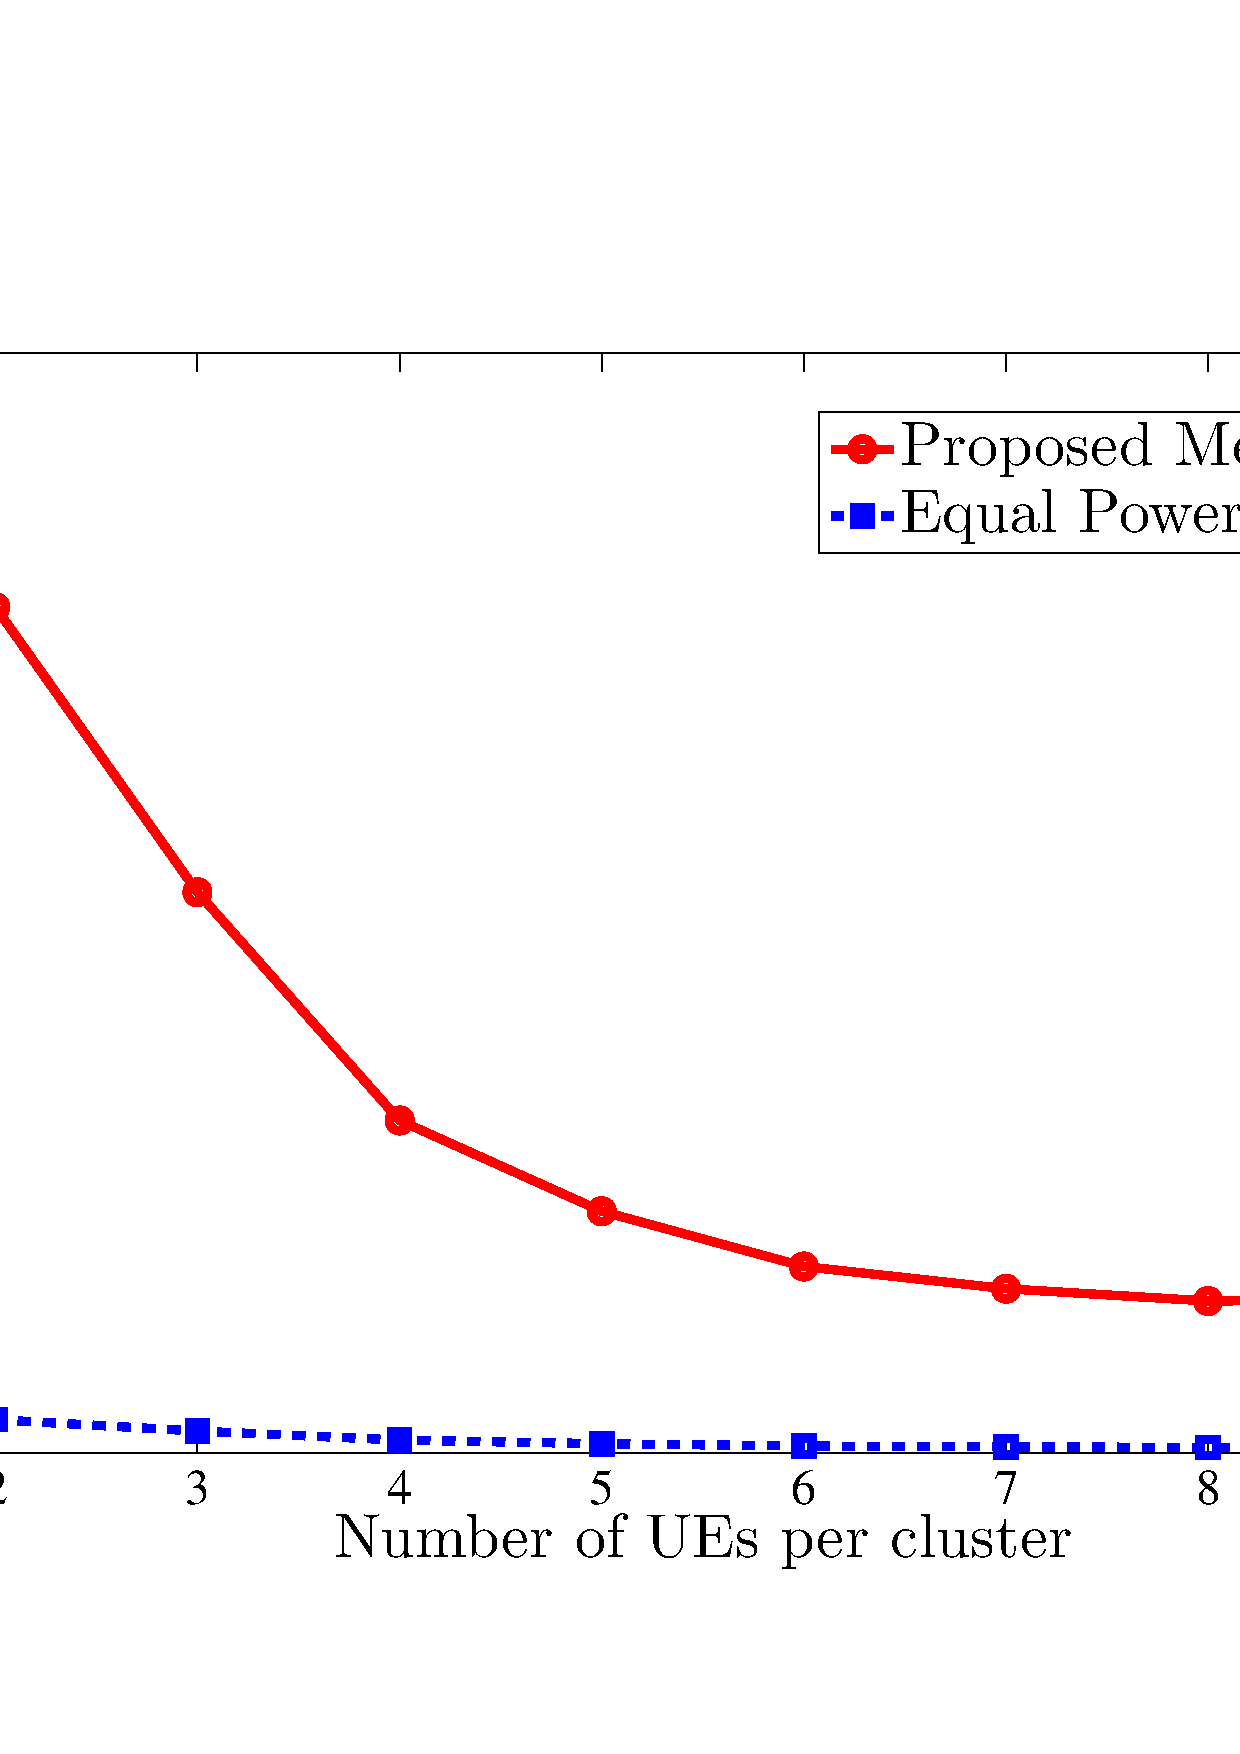
\includegraphics[width=0.5\linewidth, height=6cm]{ue}
  \caption{Energy efficiency vs number of UE for Optimized and Equal Power Allocation, plotted for parameters given in Table I with $M_s=30$.}
  \label{fig:nem2}
\end{figure}
%\bibliographystyle{ieeetr}
%\bibliography{bib1}
%\setLTRbibitems
\begin{figure}
  \centering
    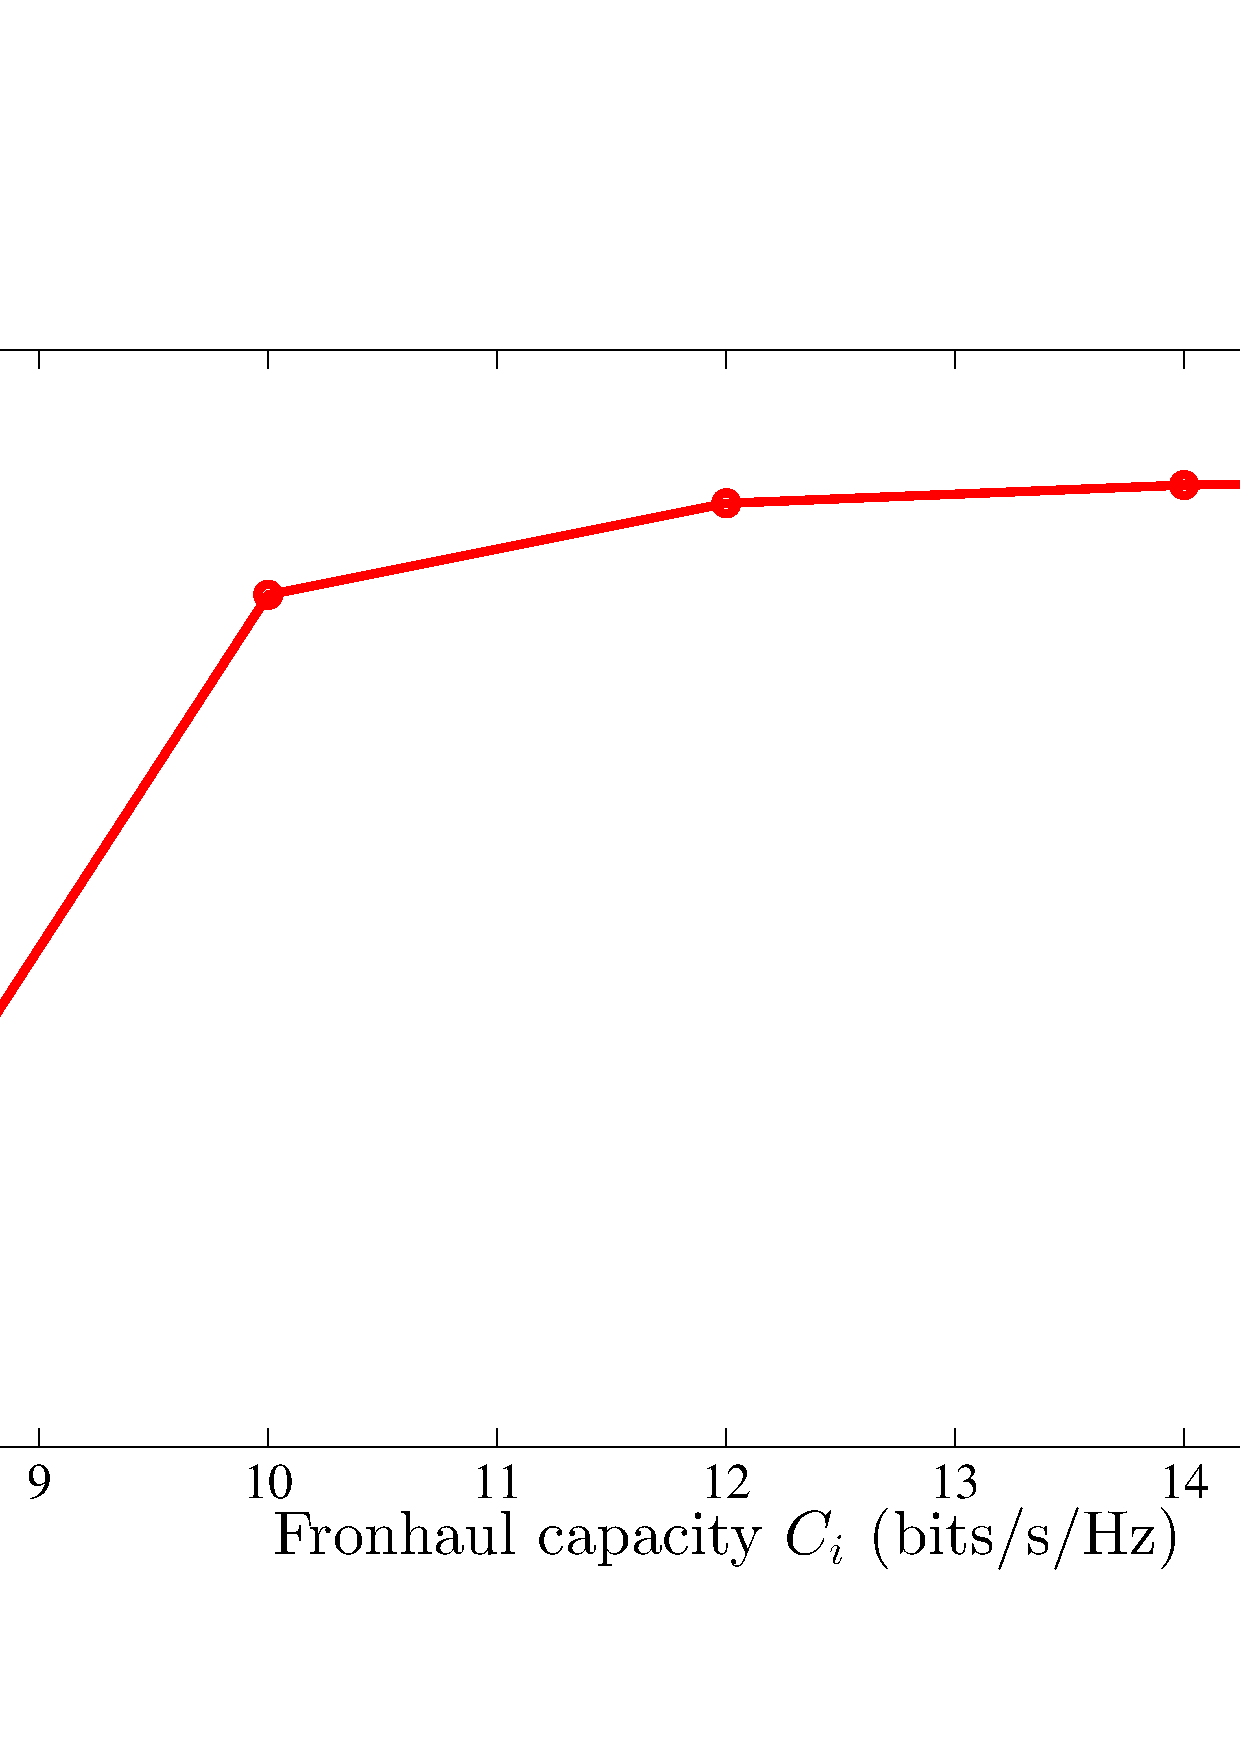
\includegraphics[width=0.5\linewidth, height=6cm]{c}
  \caption{Energy efficiency vs ${C}^{th} $ constraint with $S =3$, $Ms= 20$, $U =3$. }
  \label{fig:nem3}
\end{figure}


In Fig. \ref{fig:nem3}, EE is depicted as a function of the maximum fronthaul link capacity constraint. It could be understood from the figure that, as the capacity exceeds 12 (bits/s/Hz), the increase in the fronthaul capacity does not affect energy efficiency significantly, since the achievable rate is limited by the wireless channel between RRHs and UEs.
\section{Conclusion}
The project has focused on addressing the optimal power allocation in downlink of a MIMO C-RAN system with limited fronthaul capacity.
The system model is expressed and the equivalent problem of maximizing the EE is solved by using an iterative algorithm and Lagrangian function.
Simulation results demonstrate that the proposed algorithm outperforms the equal power allocation. It is also shown that by increasing the number of RRHs in each cluster, the performance of the system would be enhanced, and increasing the number of UEs in each cluster reduces the system performance.

\newpage
\bibliographystyle{ieeetr}
\bibliography{m}
 %%
\
\end{document}
